% coming soon

We have implemented our switching continual approach in the MAPSIM
environment~\cite{brenner:nebel:jaamas09},
using \system{dlib-ml}~\cite{king:2009} for belief
revision. Sequential sessions use a modified version of Fast
Downward~\cite{fast-downward}, and DT sessions use our own fast
contingent procedure. We also implemented a simple dual-mode
replanning {\em baseline} approach in MAPSIM. Here, a DT session
executes a single greedy entropy reduction action, wrt to active
assumptions, when a switching action is scheduled for execution,
returning control to a new sequential session.


To test our approach we use a robot exploration domain based on a
scenario from our physical robotic system. Here, a robot is exploring
an office or living environment, and trying to report the locations of
objects to their owner. Basic types are {\tt rooms}, {\tt places} and
{\tt objects}. Places are topological map nodes that occur in rooms.
Objects, and also the robot, are always located at a place. The robot
can move around the rooms via connections between places given by a
{\tt connected} predicate. Each room has a, possibly unknown, {\em
  category} (e.g. kitchen, office, living room). Certain objects are
more likely to be located in rooms of a particular category.  For
example, a box of cornflakes is more likely to be located in the
kitchen than the office. The robot can look for an object at a place
by executing a {\tt look-for-object} action. Executing {\tt
  look-for-object} results in a noisy sensing outcome, sometimes
indicating a positive perception if the object is there. We have that
some objects are harder to detect than others. Finally, if the robot
is in the presence of a human, it can ask what type of room it is
currently in, however conducting a dialogue is more costly than
running a vision algorithm (cost of 8 vs costs of 3).

%%  Therefore, an instantaneous positive detection of an object is
%% not proof positive of it being there.

We evaluated our switching planner against the {\em baseline} in several
tasks with the number of rooms ranging from 3 to 6. We examine the
impact of sensing reliability, experimenting using sensor models that
are: ({\em reliable}) $0.9$ chance the object is perceived if it is
present, ({\em semi-reliable}) chance is 0.65, and ({\em noisy})
chance is 0.4. The continual planning times are reported in
Figure~\ref{fig:results-time}, and the quality data in
Figure~\ref{fig:results-quality}. Here, in switching runs we examine
the performance of our system where $b_0$ allocates non-zero
probability to between 20 and 200 abstract states during contingent
sessions. For Item~$a$-$e$ the objective is to find one or more
objects and report their position to the user. In some of the tasks we
configured the environment so that no plan exists, by excluding the
desired object from the environment. Item~$f$ reports for tasks
requiring indirect sensing, where the robot must relocate to a
particular room category. For Item~$f$ there is no human in the
environment, and therefore the {\em baseline} cannot be used, because there
are no sensing schemata that directly sense room categories. In our
evaluation we run 50 simulations in each configuration, and have a
timeout on each simulation of 30 minutes (1800 seconds)\footnote{All
  experiments were conducted on a 2.3GHz AMD Opteron using one CPU
  core.}. In our domain, rewards encapsulate a goal condition, and
therefore we find it intuitive to report average costs of the plans
and the success rate in problems that admit a solution (i.e., positive
reward scaled by a constant factor).

%% Because the switching utility model 

%% Using a satisficing, optimistic serial planner in sequential sessions
%% makes optimising for the expected reward difficult. Only reasoning
%% about single traces, it is optimistic wrt the remaining costs to a
%% goal and pessimistic regarding the probability of reaching it. By
%% setting the rewards to non-extremal values has little effect on that
%% system. Therefore, we do not consider expected utility in our
%% experiments. Instead, we report average costs of the plans and the
%% success rate (as a ratio between solved and solvable problems).

\begin{figure}[h!]
  % \centering
  % 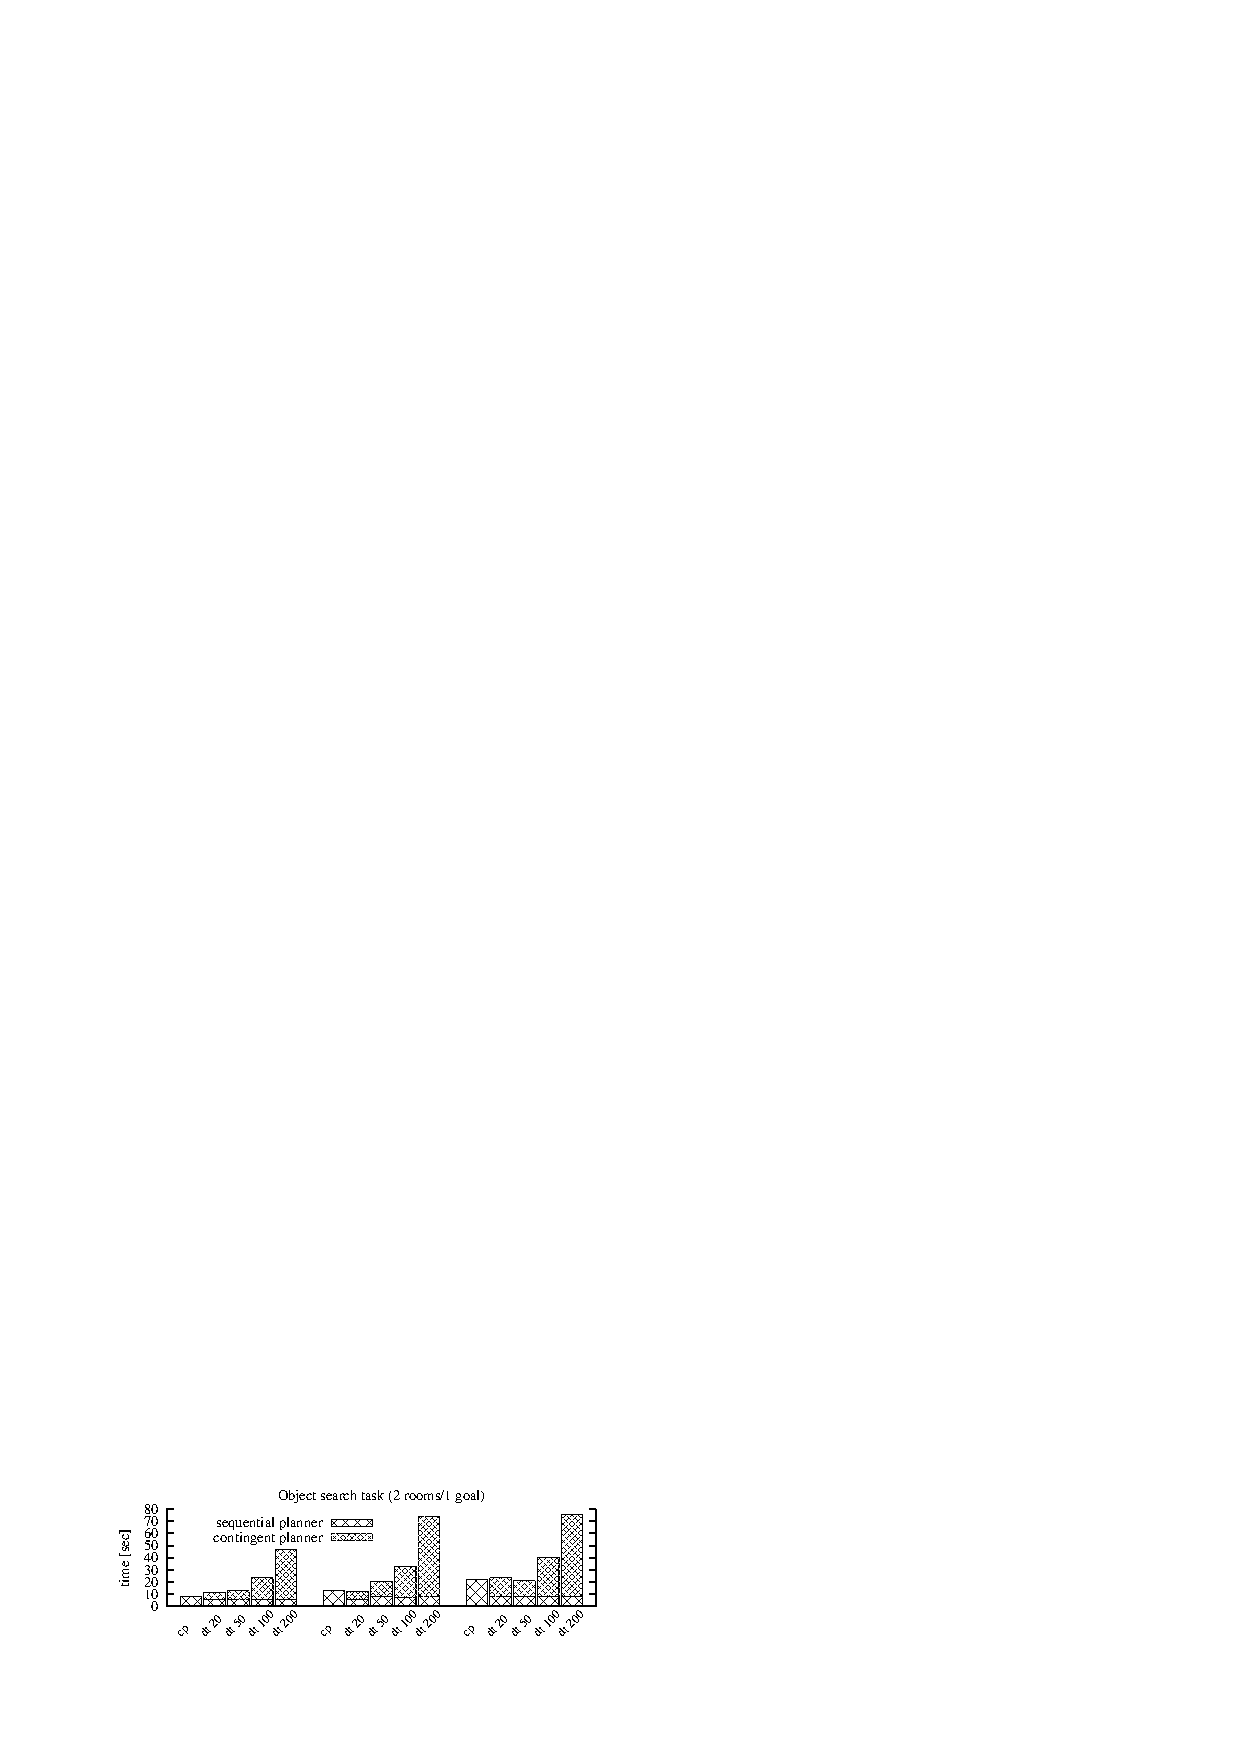
\includegraphics{dora1-time}\hfill
  % \vspace{2mm}
  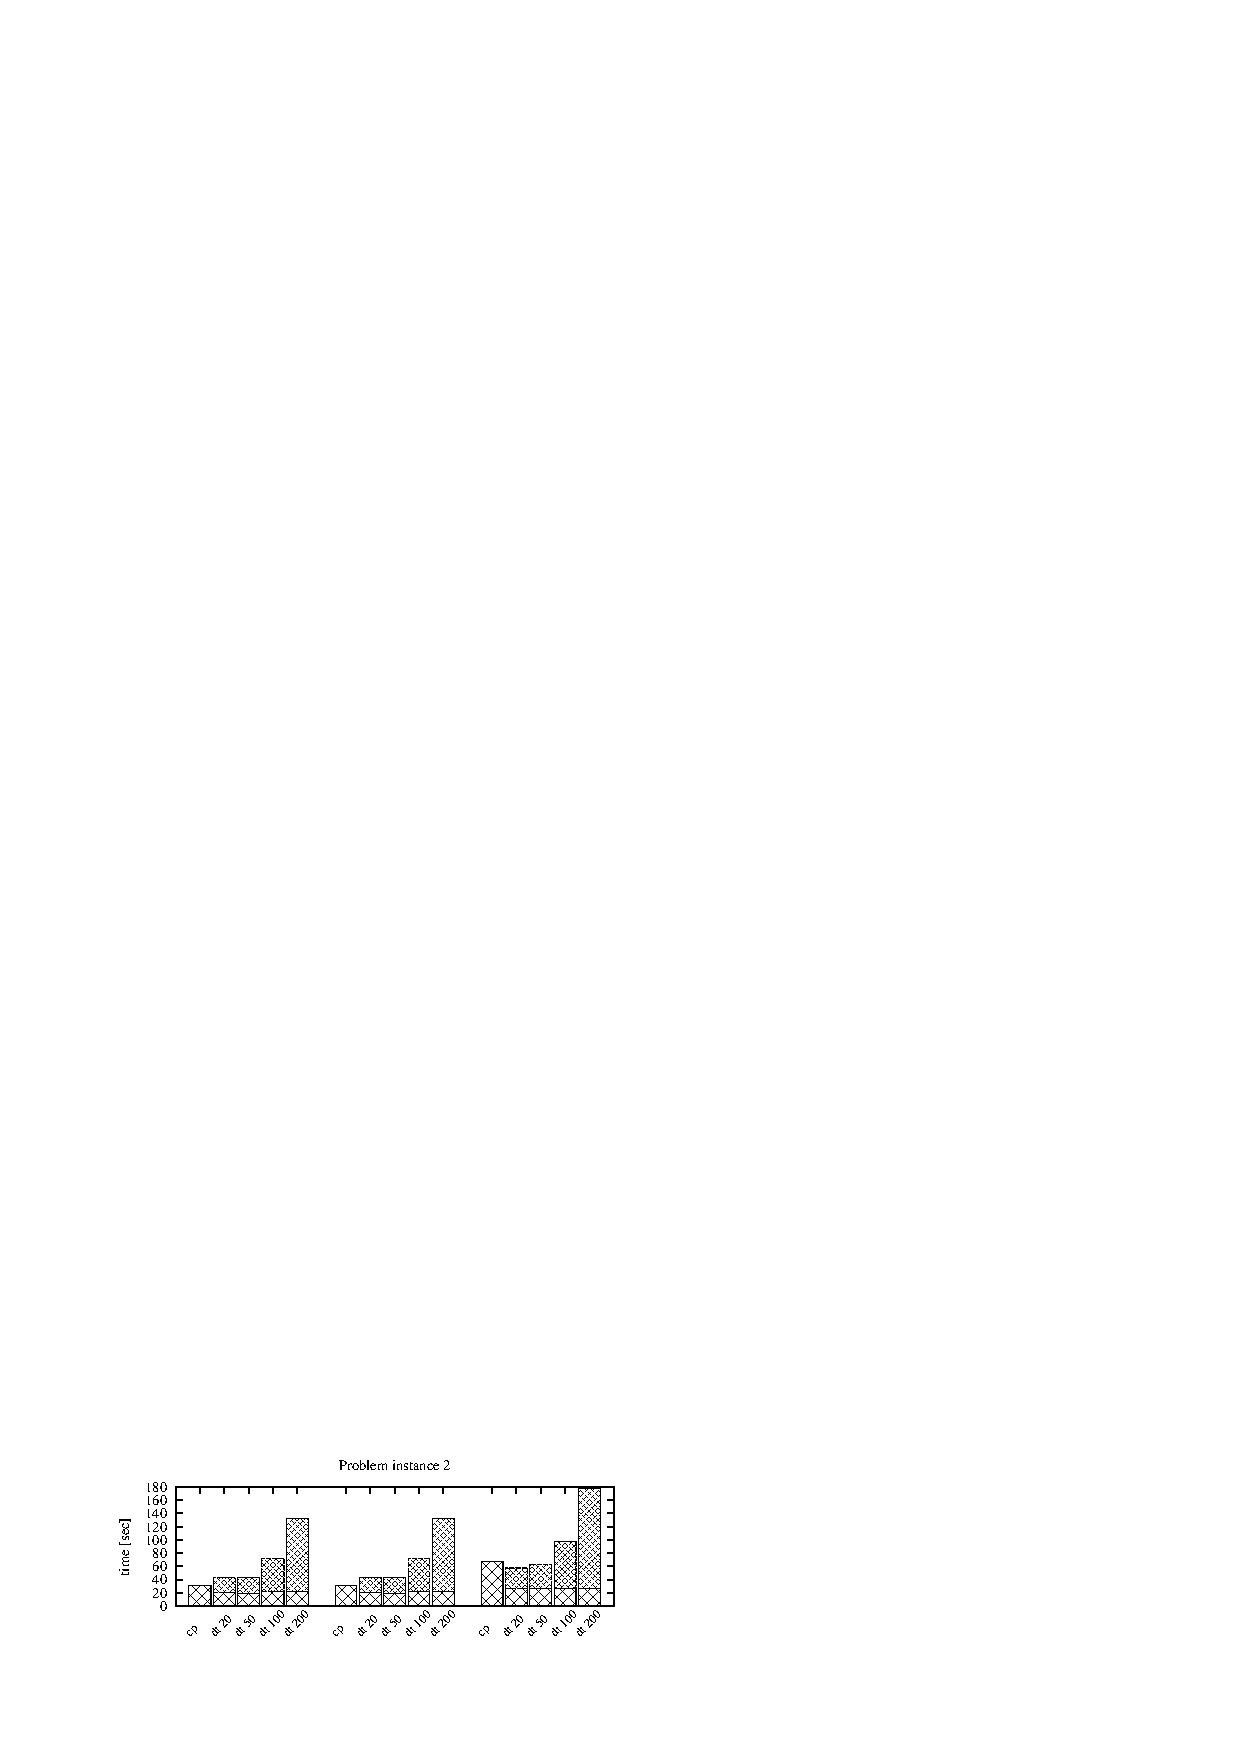
\includegraphics{dora2-time}\hfill
  % \vspace{2mm}
  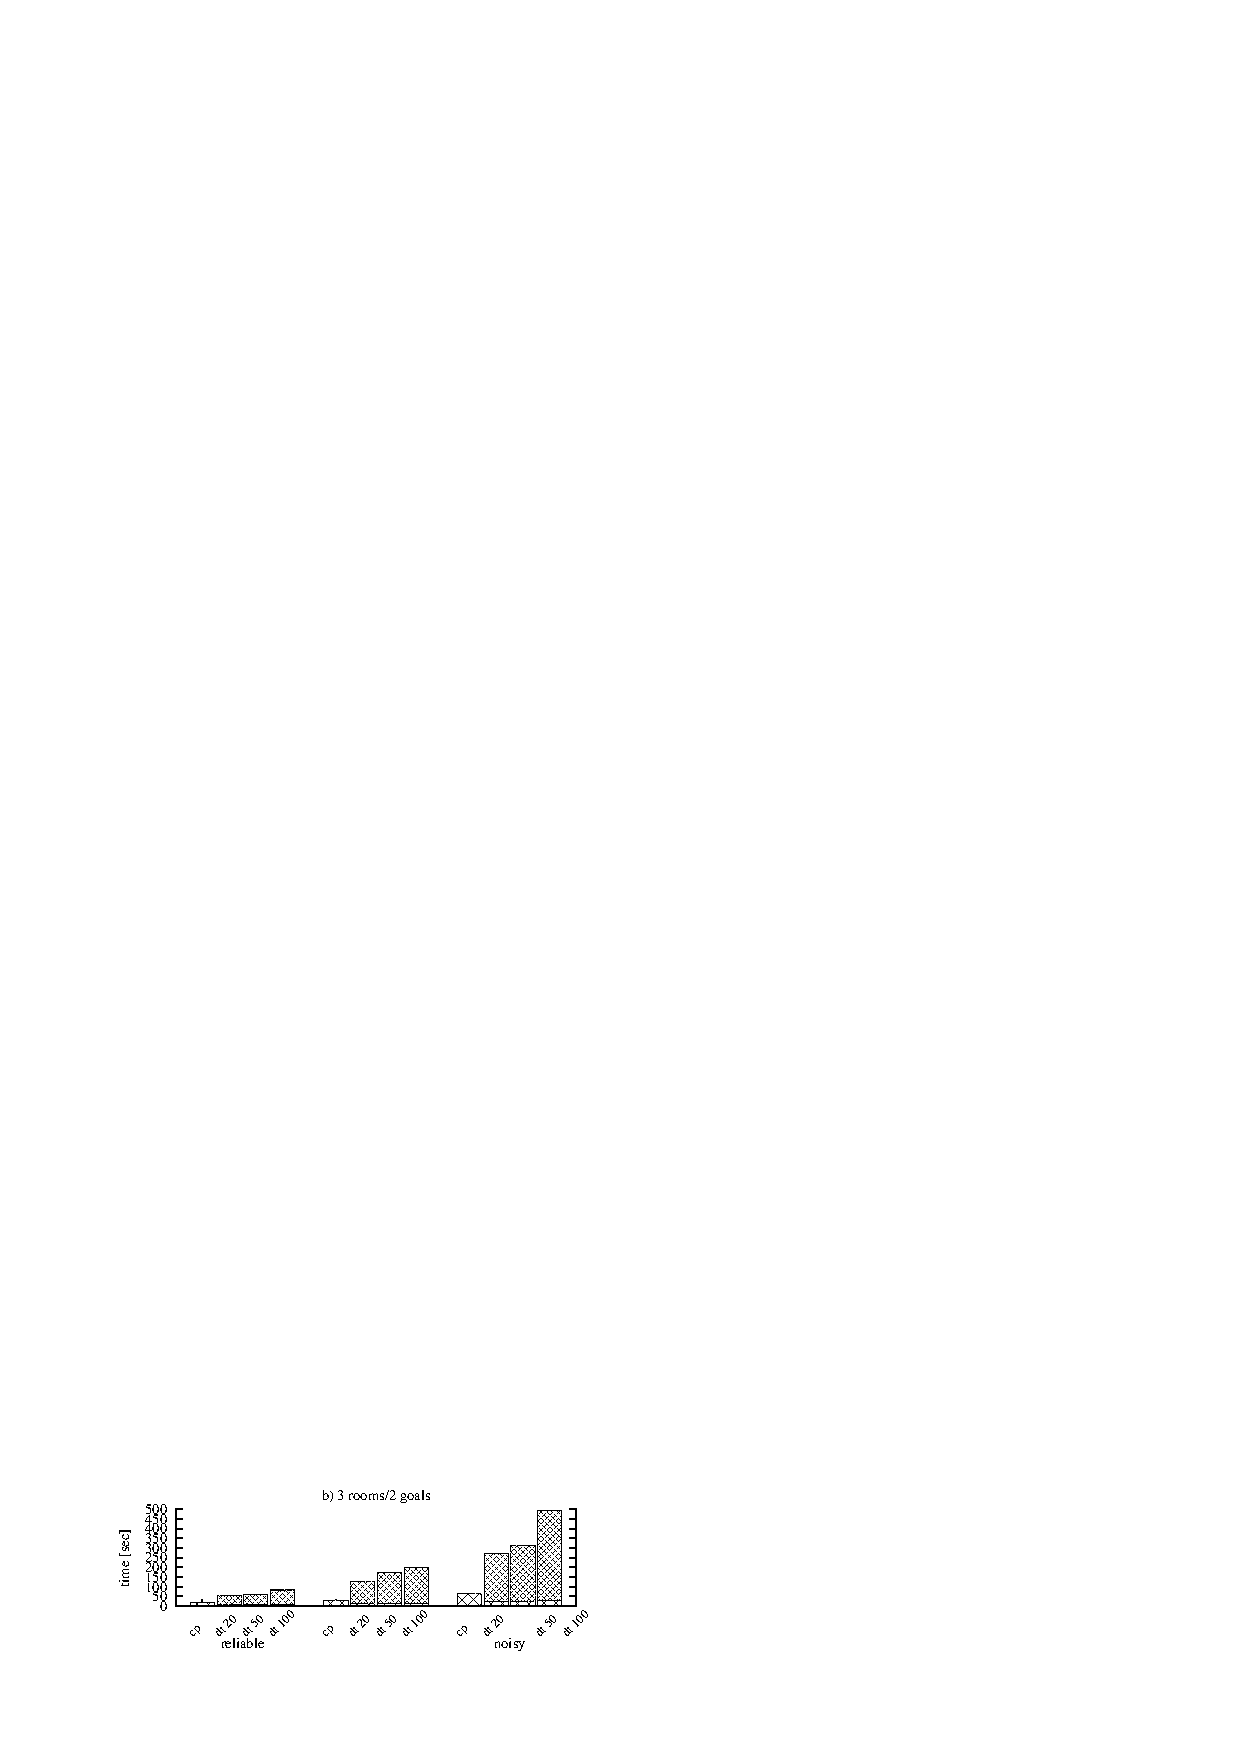
\includegraphics{dora3-time}\hfill
  % \vspace{2mm}
  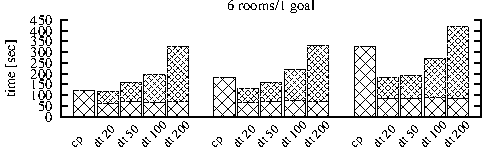
\includegraphics{dora4-time}\hfill
  \vspace{2mm}
  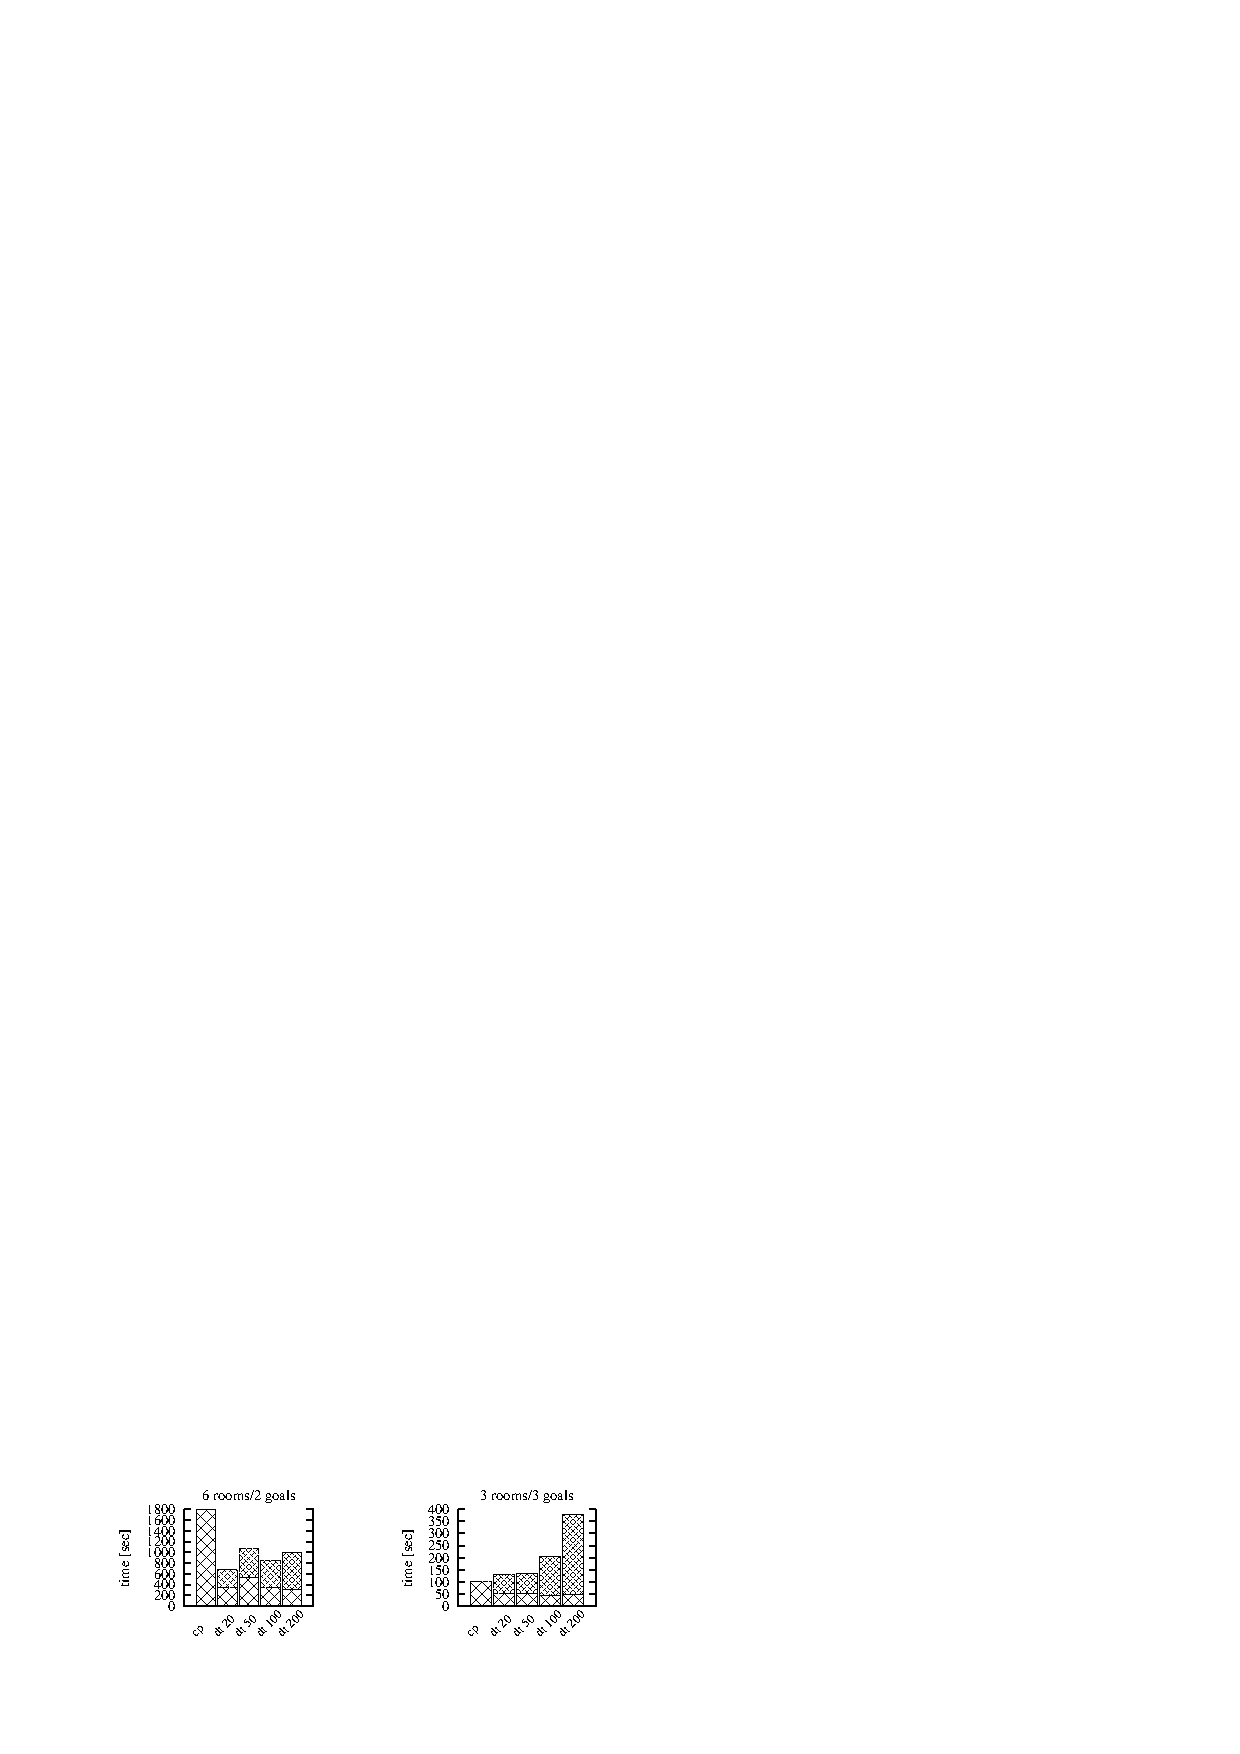
\includegraphics{dora56-time}\hfill
  \vspace{2mm}
  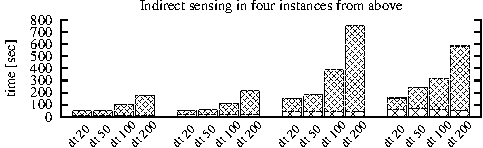
\includegraphics{dora-cat-time}\hfill
  \caption{Average runtime}
  \label{fig:results-time}
\end{figure}

\begin{figure}[h!]
  % \centering
  % 
\includegraphics{dora1-quality}\hfill
  % \vspace{2mm}
  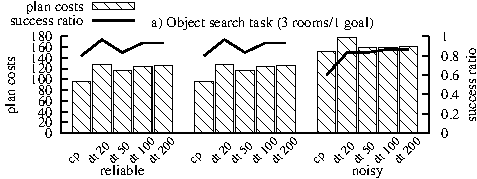
\includegraphics{dora2-quality}\hfill
  % \vspace{2mm}
  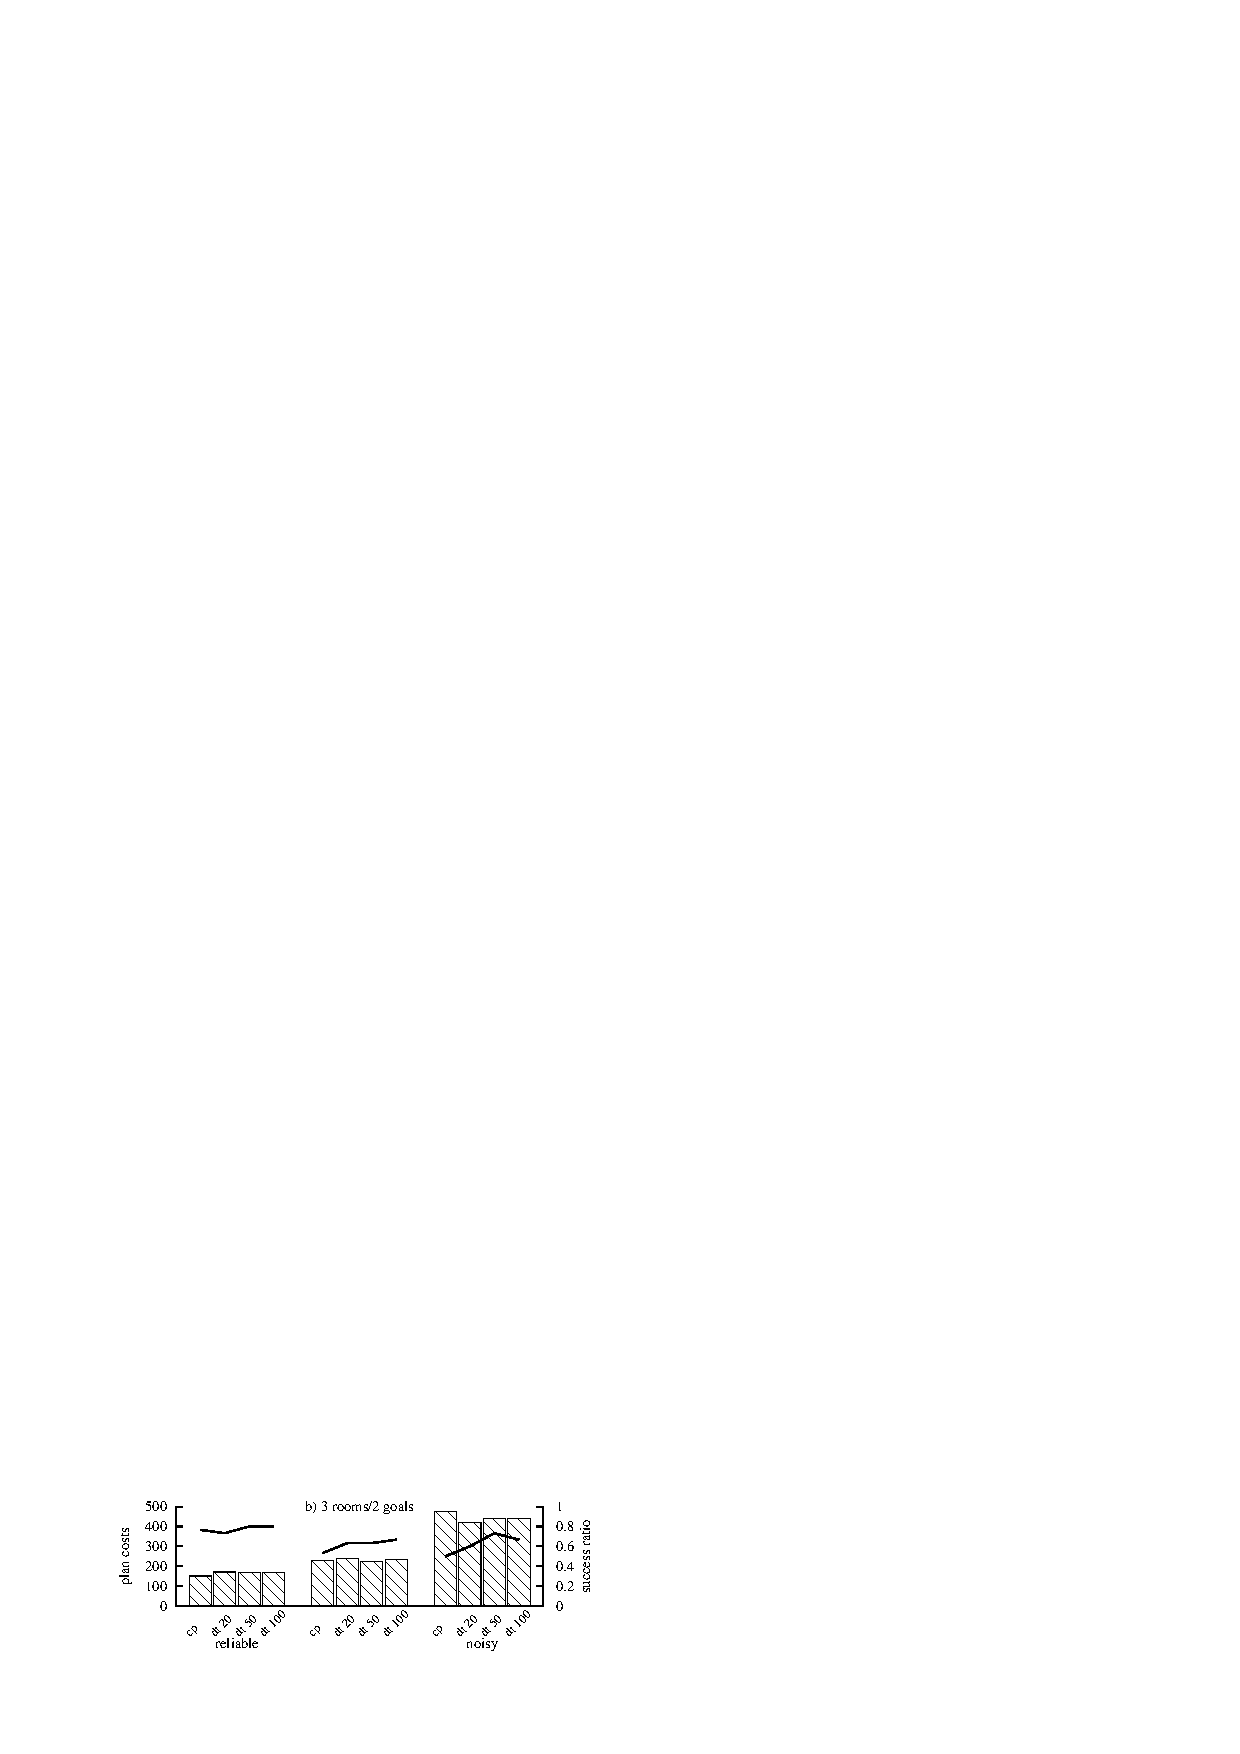
\includegraphics{dora3-quality}\hfill
  % \vspace{2mm}
  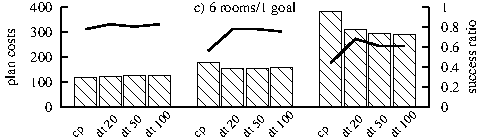
\includegraphics{dora4-quality}\hfill
  \vspace{2mm}
  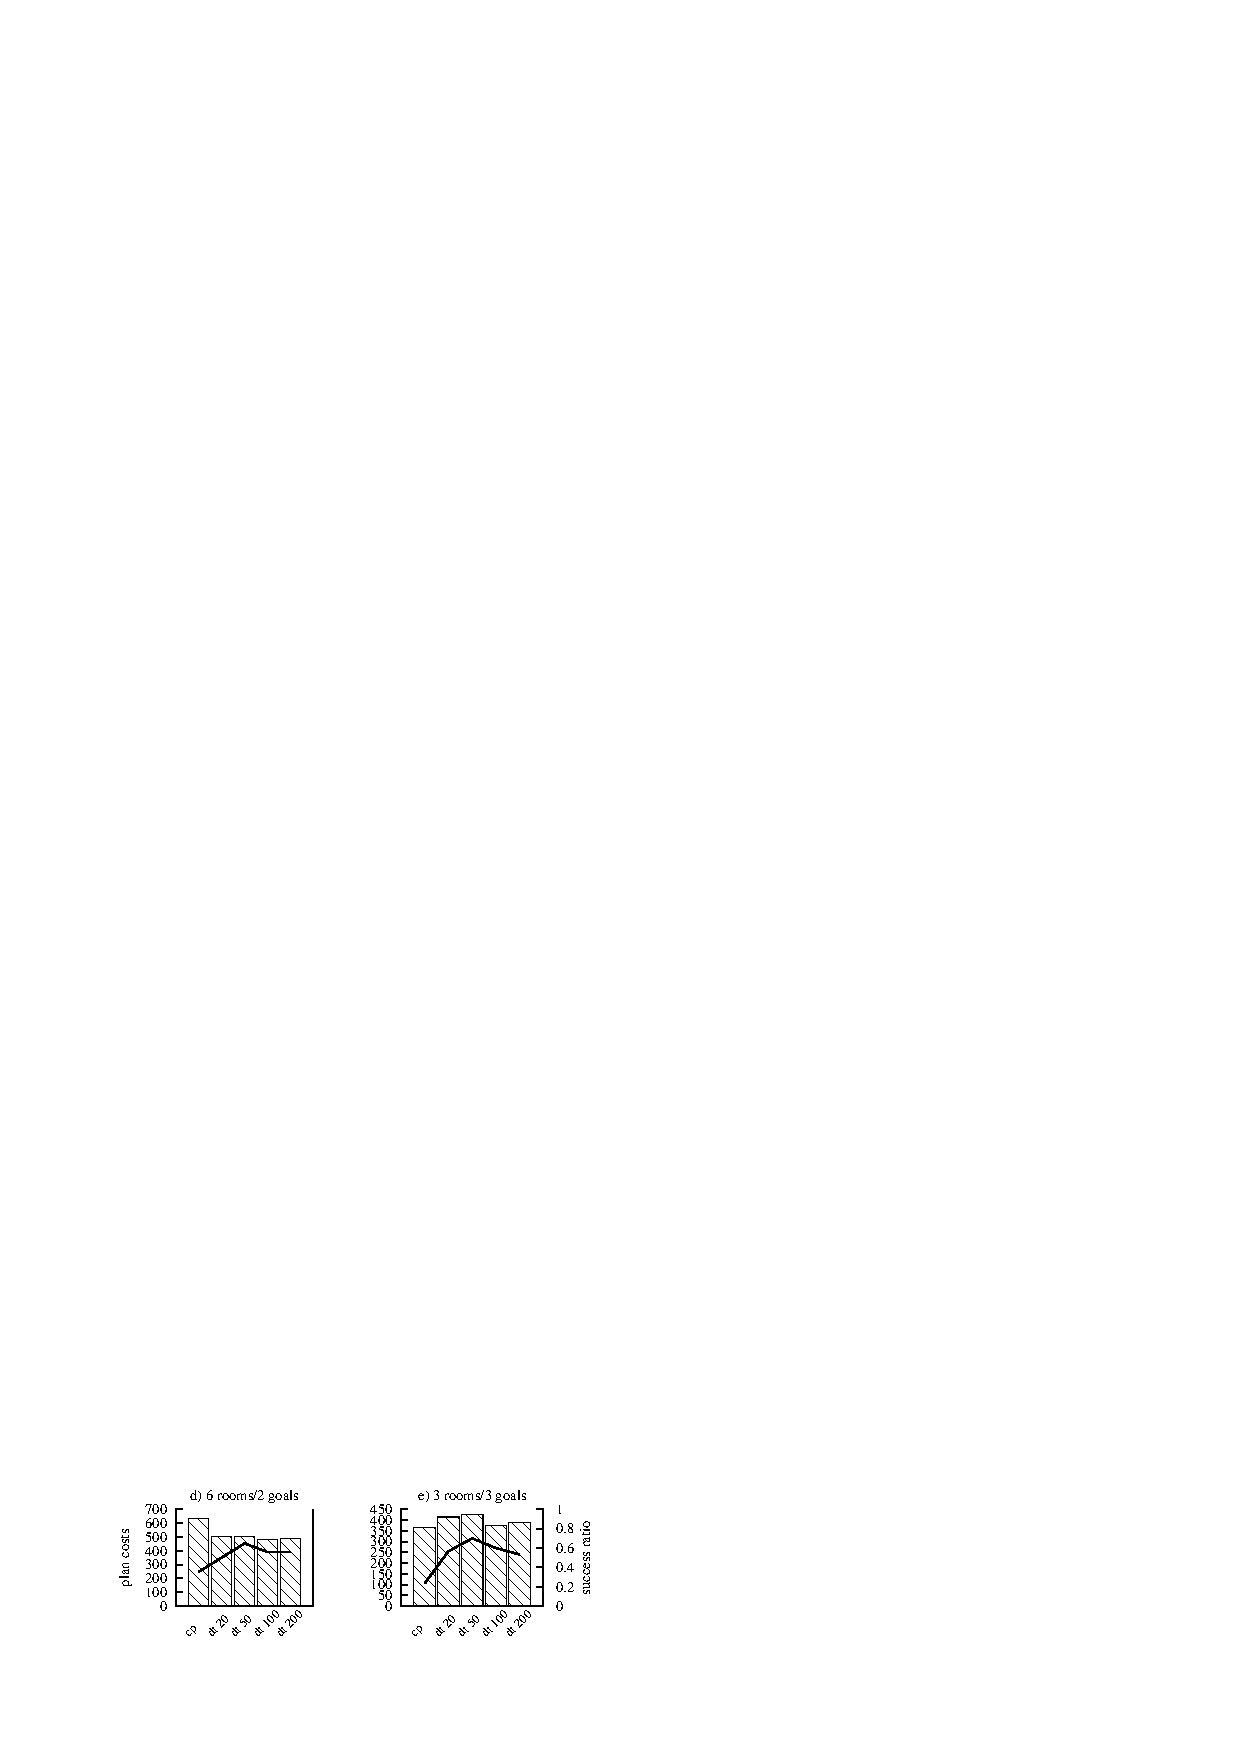
\includegraphics{dora56-quality}\hfill
  \vspace{2mm}
  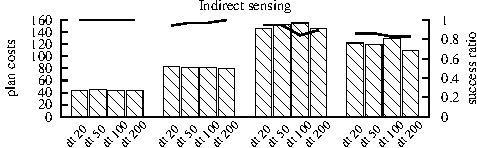
\includegraphics{dora-cat-quality}\hfill
  \caption{Average plan costs and number of successful runs.}
  \label{fig:results-quality}
\end{figure}



Examining success ratios and plan costs, where sensing is reliable
there is little to be gained by using the contingent planner, as the
greedy sensing approach of the {\em baseline} is sufficient. Not
surprisingly, as sensing degrades contingent planning pays off.  Also,
we find that time spent in contingent planning increases steeply as
the abstraction $\bstate_0$ becomes more refined.  That refinement
seems to be paying off in terms of the success ratio, particularly for
tasks $d$ and $e$, where we had sequential sessions using weighted
$A^*$ (rather than $A^*$). For less refined initial configurations,
the increase cost of contingent planning is compensated by a decrease
in Fast Downward planning times. The relatively high success rate
irrespective of the level of refinement in the initial configuration
indicates the effectiveness of using conditional entropy to guide
abstraction refinement in our setting.
